\chapter[Diseño de la Plataforma]{Diseño de la Plataforma}
\label{Chap4}

La arquitectura planteada en la figura \ref{fig:ej9} es simple y fácil de implementar, pues scrapy mismo puede insertar los datos scrapeados de las web de forma directa en PostGreSQL, aunque presenta un problema. Djando hace uso de un sistema de gestión de versiones de los cambios realizados en la BBDD con el fin de reducir la carga de peticiones a la BBDD, esto se aplica desde el lado de Django, lo que supondría un problema a la hora de insertar datos directamente de Scrapy a PostGreSQL, pues los nuevos datos no serán detectados por Django, generando la situación de que una vez se vayan a pedir los nuevos datos, Django no devuelva nada, pues desde su punto de vista los datos anteriormente pedidos son la versión mas reciente, luego no es necesario realizar llamada alguna a la BBDD.

\begin{figure} [H]
	\centering
	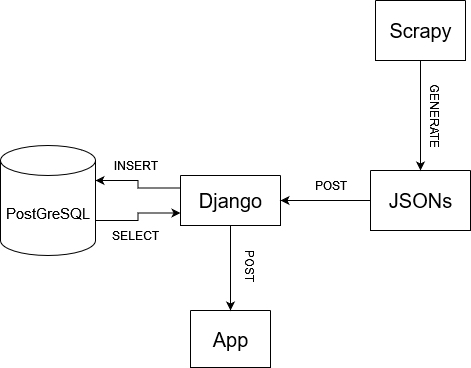
\includegraphics[width=0.4\textwidth]{fig/estructura_usada.png}
	\caption[Estructura de datos usada en el proyecto]{Estructura usada}
	\label{fig:ej10}
\end{figure}

Pasa solventar el problema, inicialmente se encontró el pluggin scrapy\_djangoitem, promete la comunicación entre scrapy y Django, pero se decidió no usarlo al llevar siete años sin revisiones. Como alternativa, se ha optado por la arquitectura de la figura \ref{fig:ej10}, que incluye un paso intermedio al almacenar los datos obtenidos de las distintas webs en formato JSON, para posteriormente enviárselos a Django, el cual se encargara de subir los datos a la BBDD.

\section{Trabajar con los Datos}

\begin{lstlisting}[caption={Flujo de obtencion y tratamiento de los datos}, label=cod:112]
	Pedir datos
	Formatear datos
	Mandar datos a la BBDD
	Marcar datos como old
	
	While(true)
		Pedir datos
		Formatear datos
		Filtrar datos
		Mandar datos a la BBDD
		Marcar datos como old
\end{lstlisting}

El flujo que realizan los datos es el mostrado en el código \ref{cod:112}, inicialmente se pedirán los datos, como los datos obtenidos no son los mismos para cada web, se formatean para compartir una estructura heterogénea, en caso de ser la primera iteración, se mandan directamente los datos a la BBDD, de no ser la primera iteración, se filtran los nuevos datos de aquellos mascados como old (viejo), se envían los datos a la base de datos y, una vez enviados son marcados como old para ser el punto de comparación respecto a los datos que se obtendrán en la próxima iteración.

\subsection{Formato de Datos}
No todas las webs presentan sus datos de la misma manera, es por eso que los datos a obtener pueden llegar a estar repartidos en distintas páginas, haciendo necesario el uso de múltiples Spiders, resultando en múltiples JSON. A su vez, cada web esta especializada en unos tipos de datos en concreto, lo que hace que el JSON resultante de cada web difiere en formato.\newline
\newline
Debido a ello, para cada web se ha creado una función para parsear (formatear) los datos obtenidos, de esta manera se dispone de una estructura única para los datos recibidos, haciendo su uso posterior más fácil, ya sea a la hora de tratarlos como para almacenarlos en la base de datos. El esquema obtenido se observa en el código \ref{cod:113}.

\begin{lstlisting}[language=json, basicstyle=\small, label=cod:113]
[
{
	"coordenadas": "X. 598270,3 | Y. 4659333 | Z. 37928",
	"estacion": "64",
	"datos": [
	{
		"fecha y hora": "01/06/2023 11:20:00",
		"temperatura (C)": null,
		"humedad (%)": null,
		"precipitacion (mm)": null,
		"nivel (m)": "0,05",
		"caudal (m^3/s)": null,
		"radiacion (W/m^2)": null
	}
	]
}
]
\end{lstlisting}

\subsection{Filtrado de Datos}
A fin de reducir la carga a la base de datos, los JSON resultantes del proceso de formateo, son filtrados mediante la comparación con los ficheros anteriormente marcados como old, de esta forma, nos aseguramos de mandar a la base de datos unicamente las instancias nuevas de los datos recogidos, pues no disponemos de ninguna manera de filtrar los datos a la hora de obtenerlos. Estos datos serán guardados en un tercer JSON.

\section{Arquitectura}
Llevando a delante el trabajo, se ha diseñado la arquitectura de la figura \ref{fig:ej7}.

\begin{figure} [h]
	\centering
	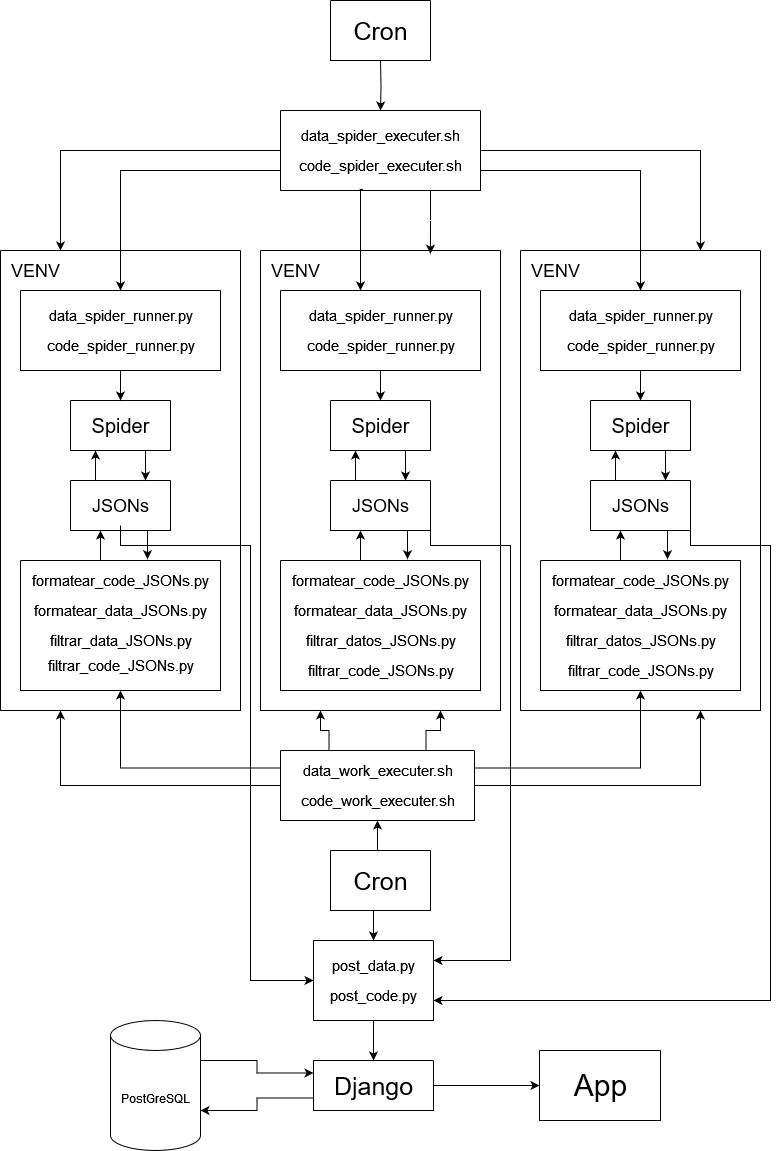
\includegraphics[width=0.7\textwidth]{fig/arquitectura.png}
	\caption[Arquitectura de obtención y tratamiento de datos]{Arquitectura de obtención y tratamiento de datos}
	\label{fig:ej7}
\end{figure}

\subsection{Entornos virtuales}
Con el fin de que la plataforma sea lo mas fácilmente ampliable, se ha decidido que cada Spider disponga de su propio entorno virtual, esto permite añadir dependencias de tal forma que no afecten a el resto de los scripts presentes, ayudando en la encapsulación de dependencias.\newline
\newline
Actualmente la plataforma dispone de cuatro entornos virtuales para cada Spider y un entorno virtual sobre el que ejecutar el servidor de Django.

\subsection{Spiders}
Cada Spider representa una web, de tal forma que cada una de ellas obtiene los datos de la web sobre la que se ha diseñado exclusivamente, para poder realizar esta tarea por cada web han sido necesarias varias Spider, aunque de forma simplificada se pueden agrupar por, aquellas que obtienen las estaciones junto con sus códigos y, las de obtención de datos. De esta forma, se dividen las tareas con la posibilidad de ejecutar aquella que mejor venga en cada momento.

\subsection{Runners}
Runner es la forma en la que han sido nombrados los Scripts cuya función es posibilitar la ejecución en nuestro caso asíncrona de una o múltiples Spiders mediante un único comando. Es un Script simple en el que una vez dispones de la estructura básica en caso de necesitar añadir o eliminar una Spider solo tienes que agregar o eliminar la Spider en cuestión y ya estaría listo.\newline
\newline
A su vez, al añadir un intermediario el comando de ejecución pasa de ser, scrapy crawl nombreSpider por cada Spider que se desea ejecutar, a, python nombreRunner.py facilitando la automatización de ejecución de las Spider.

\subsection{Executers}
Aumentado un poco mas la abstracción nos encontramos con los Executers, Scripts en Bash encargados de activar el entorno virtual de la Spider deseada y acto seguido ejecutar su respectivo Runner.\newline
\newline
Estos existen (en mayor medida que los Runners) con el fin de ayudar con el mantenimiento de la arquitectura, creando un nuevo intermediario en la cadena de ejecución.\newline
\newline
Están diseñados de tal forma que funcionen pasandoles un único argumento representando la web de la que quieres obtener los datos, haciendo que la agregación de nuevas Spiders junto con sus entornos sea tan sencillo como respetar las rutas y nombres predefinidos.

\subsection{Directorios de los JSONs de datos}
Este apartado es un conjunto de directorios en los que se van almacenando los JSON obtenidos tras los distintos procesos a los que son sometidos. Los directorios en cuestión, siguiendo orden de creación para los JSON de datos son:

\begin{multicols}{2}
Directorios de los datos de estación:
\begin{enumerate}
	\item RawData
	\item ParsedData
	\item RefinedData
	\item OldData
\end{enumerate}

\columnbreak

Directorios de los códigos de estación:
\begin{enumerate}
	\item RawCode
	\item ParsedCode
	\item RefinedCode
	\item OldCode
\end{enumerate}
\end{multicols}

El primer nivel es aquel que almacena los JSON que genera la llamada con la Spider a la web. El segundo, los resultantes tras ejecutar ya sea formatear\_data\_JSONs.py en caso de querer parsear los datos o formatear\_code\_JSONs.py para los códigos. El tercero almacena los ficheros generados tras eliminar la duplicidad de datos en comparación con los ya almacenados en la base de datos, mediante la ejecución de filtrar\_data\_JSONs.py. Finalmente el cuarto guarda el fichero original ya formateado tras la comparación.

\subsection{Posts}
Estos Scripts son los encargado de enviar los datos mediante un Post Request al servidor Django. Diseñados bajo el mismo principio de fomentar la ampliabilidad del proyecto que los Executer, reciben el nombre de la web de la cual deseas enviar los datos a la hora de ejecutarlo junto al comando en forma de argumento.

\subsection{Cron}
Cron es un administrador regular de procesos en segundo plano presente en los sistemas basados en Unix. Con el es posible programar la automatización de ejecución de procesos en intervalos de tiempo, pudiendo indicar el minuto, hora, día, mes e incluso día de la semana.\newline
\newline
La especificación de los procesos se realiza en el archivo crontab y, su estructuración es la siguiente:

\begin{verbatim}
.--------------- minuto (0-59) 
|  .------------ hora (0-23)
|  |  .--------- día del mes (1-31)
|  |  |  .------ mes (1-12) o meses en inglés
|  |  |  |  .--- día de la semana (0-6) (domingo=0 o 7) o días en inglés 
|  |  |  |  |
*  *  *  *  *  comando a ejecutar
\end{verbatim}

Para este proyecto se quiere el equivalente a dos instancias de Cron, una que se encargue de obtener los datos ya sea cada quince minutos, media hora y una hora manteniendo la base de datos actualizada para poder realizar las posteriores predicciones y, otra que mensualmente compruebe la existencia de nuevas estaciones o el cese del uso de alguna de las ya disponibles.\newline
\newline
Así pues, Cron es el encargado de ejecutar cada proceso necesario dentro de la plataforma, ya sea, ejecutar las Spiders, los Scripts de formateo como de filtrado y, el envío de los datos a Django para su inserción en PostGreSQL. De esta forma dispondríamos de un sistema cerrado automático, el cual nos permitiría trabajar en otros apartados como puede ser la integración de mas webs en la plataforma o la mejora del sistema de predicción.

\subsection{API Django}
La instancia del servidor de Django es la encargada de tanto recibir los datos obtenidos como de enviarlos a la base de datos. Finalmente, una vez se dispusiera de una aplicación de predicción, se encargaría de pedir los datos almacenados y enviarlos mediante POST a la aplicación.

\subsection{Base de datos PostGreSQL}

\begin{figure} [H]
	\centering
	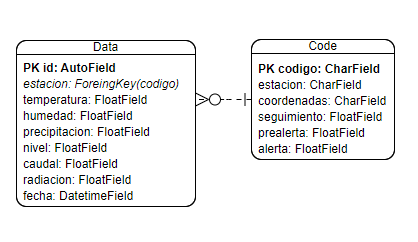
\includegraphics[width=0.7\textwidth]{fig/TablasBBDD.png}
	\caption[Tablas de la base de datos]{Tablas de la base de datos}
	\label{fig:ej33}
\end{figure}

Las tablas de la figura \ref{fig:ej33}, tienen una relación uno a muchos, siendo el campo estacion de la tabla Data la ForeingKey usada. Para la tabla Data, al almacenar miles de datos, se ha optado por usar una PrimaryKey auto incremental. A su vez, a excepción del campo fecha, cualquiera de los campos pueden ser nulos, pues cada web proporciona unicamente un conjunto de los datos. En la tabla Code, exceptuando la clave primaria y el nombre de la estación, el resto de campos tienen la posibilidad de ser nulos.
